%% For double-blind review submission, w/o CCS and ACM Reference (max submission space)
\documentclass[sigplan,review]{acmart}\settopmatter{printfolios=true,printccs=false,printacmref=false}
%% For double-blind review submission, w/ CCS and ACM Reference
%\documentclass[sigplan,review,anonymous]{acmart}\settopmatter{printfolios=true}
%% For single-blind review submission, w/o CCS and ACM Reference (max submission space)
%\documentclass[sigplan,review]{acmart}\settopmatter{printfolios=true,printccs=false,printacmref=false}
%% For single-blind review submission, w/ CCS and ACM Reference
%\documentclass[sigplan,review]{acmart}\settopmatter{printfolios=true}
%% For final camera-ready submission, w/ required CCS and ACM Reference
%\documentclass[sigplan]{acmart}\settopmatter{}


%% Conference information
%% Supplied to authors by publisher for camera-ready submission;
%% use defaults for review submission.
%\acmConference[FTfJP'19]{Workshop on on Formal Techniques for Java-like Programs}{July 15--19, 2019}{London, United Kingdom}
\acmConference[]{}{}{}
\acmYear{2019}
\acmISBN{} % \acmISBN{978-x-xxxx-xxxx-x/YY/MM}
\acmDOI{} % \acmDOI{10.1145/nnnnnnn.nnnnnnn}
\startPage{1}

%% Copyright information
%% Supplied to authors (based on authors' rights management selection;
%% see authors.acm.org) by publisher for camera-ready submission;
%% use 'none' for review submission.
\setcopyright{none}
%\setcopyright{acmcopyright}
%\setcopyright{acmlicensed}
%\setcopyright{rightsretained}
%\copyrightyear{2018}           %% If different from \acmYear

%% Bibliography style
\bibliographystyle{ACM-Reference-Format}
%% Citation style
%\citestyle{acmauthoryear}  %% For author/year citations
%\citestyle{acmnumeric}     %% For numeric citations
%\setcitestyle{nosort}      %% With 'acmnumeric', to disable automatic
                            %% sorting of references within a single citation;
                            %% e.g., \cite{Smith99,Carpenter05,Baker12}
                            %% rendered as [14,5,2] rather than [2,5,14].
%\setcitesyle{nocompress}   %% With 'acmnumeric', to disable automatic
                            %% compression of sequential references within a
                            %% single citation;
                            %% e.g., \cite{Baker12,Baker14,Baker16}
                            %% rendered as [2,3,4] rather than [2-4].


%%%%%%%%%%%%%%%%%%%%%%%%%%%%%%%%%%%%%%%%%%%%%%%%%%%%%%%%%%%%%%%%%%%%%%
%% Note: Authors migrating a paper from traditional SIGPLAN
%% proceedings format to PACMPL format must update the
%% '\documentclass' and topmatter commands above; see
%% 'acmart-pacmpl-template.tex'.
%%%%%%%%%%%%%%%%%%%%%%%%%%%%%%%%%%%%%%%%%%%%%%%%%%%%%%%%%%%%%%%%%%%%%%


%% Some recommended packages.
\usepackage{booktabs}   %% For formal tables:
                        %% http://ctan.org/pkg/booktabs
\usepackage{subcaption} %% For complex figures with subfigures/subcaptions
                        %% http://ctan.org/pkg/subcaption


%% Pkgs
%% =============================================================================

%% %%%%%%%%%%%%%%%%%%%%%%%%%%%%%%%%%% Style

%\usepackage{url}
%\usepackage{hyperref}
\usepackage{xspace}

%% %%%%%%%%%%%%%%%%%%%%%%%%%%%%%%%%%% Math

\usepackage{mathpartir} % inference rules

%% %%%%%%%%%%%%%%%%%%%%%%%%%%%%%%%%%% Graphics

\usepackage{tikz}
\usetikzlibrary{fit,shapes, positioning}


%% Commands
%% =============================================================================

%% Text
%% *********************************************************

\newcommand{\defemph}[1]{\textbf{#1}}

\newcommand{\jlcode}[1]{\texttt{\small#1}}
\newcommand{\jltype}[1]{\texttt{\small#1}}

\newcommand{\figref}[1]{Fig.~\ref{#1}}
\newcommand{\secref}[1]{Sec.~\ref{#1}}

\newcommand{\citemock}{\cite{bib:mock}\xspace}

%% %%%%%%%%%%%%%%%%%%%%%%%%%%%%%%%%%% BetaJulia

\newcommand{\BetaJulia}{\textsc{MiniJl}\xspace}
\newcommand{\BetaJuliaSub}{\textsc{JNomSub}\xspace}


%% General Math/PL
%% *********************************************************

%: \Alt                 -> |
\newcommand{\Alt}{~\vert~}

%% BetaJulia
%% *********************************************************

%% %%%%%%%%%%%%%%%%%%%%%%%%%%%%%%%%%% Style

%: type name (like Int)
\newcommand{\tyname}[1]{\ensuremath{\mathsf{#1}}}

%% %%%%%%%%%%%%%%%%%%%%%%%%%%%%%%%%%% Metavariables

%: \ty                  -> τ
\newcommand{\ty}{\ensuremath{\tau}\xspace}
%: \vty                 -> v
\newcommand{\vty}{\ensuremath{v}\xspace}

\newcommand{\cname}{\ensuremath{\mathit{cname}}\xspace}
\newcommand{\aname}{\ensuremath{\mathit{aname}}\xspace}

\newcommand{\Type}{\textsc{Type}\xspace}
\newcommand{\VType}{\textsc{ValType}\xspace}
\newcommand{\PVType}{\ensuremath{\mathcal{P}(\VType)}}

\newcommand{\NomH}{\textrm{NomHrc}\xspace}
\newcommand{\NomHClosure}{\textrm{NomHrc*}\xspace}


%% %%%%%%%%%%%%%%%%%%%%%%%%%%%%%%%%%% Type Constructors

%: \typair{t1}{t2}      -> t1 × t2
\newcommand{\typair}[2]{\ensuremath{#1 \times #2}}

%: \tyunion{t1}{t2}     -> t1 ∪ t2
\newcommand{\tyunion}[2]{\ensuremath{#1 \cup #2}}

%% %%%%%%%%%%%%%%%%%%%%%%%%%%%%%%%%%% Type Examples

\newcommand{\tysigned}{\tyname{Signed}\xspace}
\newcommand{\tyintsf}{\tyname{Int64}\xspace}
\newcommand{\tyinttt}{\tyname{Int32}\xspace}
\newcommand{\tyintst}{\tyname{Int16}\xspace}

\newcommand{\tynum}{\tyname{Num}\xspace}
\newcommand{\tyreal}{\tyname{Real}\xspace}
\newcommand{\tyint}{\tyname{Int}\xspace}
\newcommand{\tyflt}{\tyname{Flt}\xspace}
\newcommand{\tycmplx}{\tyname{Cmplx}\xspace}
\newcommand{\tystr}{\tyname{Str}\xspace}

%% %%%%%%%%%%%%%%%%%%%%%%%%%%%%%%%%%% Nominal Hierarchy

\newcommand{\bjdeclsub}[2]{\ensuremath{#1 \rhd #2}}
\newcommand{\bjnomsub}[2]{\ensuremath{#1\,{\rhd^*} #2}}

%% %%%%%%%%%%%%%%%%%%%%%%%%%%%%%%%%%% Interpretation

\newcommand{\interpty}[1]{\ensuremath{\llbracket #1 \rrbracket}}



\begin{document}

%% Title information
\title[Tag-Based Semantic Subtyping]{Decidable, Tag-Based Semantic Subtyping \\
%	to a Dynamically Typed Language} %with Nominal Types}
	for Nominal Types, Tuples, and Unions}
                                        %% [Short Title] is optional;
                                        %% when present, will be used in
                                        %% header instead of Full Title.
%\titlenote{with title note}             %% \titlenote is optional;
                                        %% can be repeated if necessary;
                                        %% contents suppressed with 'anonymous'
%\subtitle{Subtyping of Nominal Types, Pairs, and Unions}
                                        %% \subtitle is optional
%\subtitlenote{with subtitle note}       %% \subtitlenote is optional;
                                        %% can be repeated if necessary;
                                        %% contents suppressed with 'anonymous'


%% Author information
%% Contents and number of authors suppressed with 'anonymous'.
%% Each author should be introduced by \author, followed by
%% \authornote (optional), \orcid (optional), \affiliation, and
%% \email.
%% An author may have multiple affiliations and/or emails; repeat the
%% appropriate command.
%% Many elements are not rendered, but should be provided for metadata
%% extraction tools.

%% Author with single affiliation.
\author{Julia Belyakova}
%\authornote{with author1 note}          %% \authornote is optional;
                                        %% can be repeated if necessary
\orcid{nnnn-nnnn-nnnn-nnnn}             %% \orcid is optional
\affiliation{
%  \position{Position1}
%  \department{Khoury College of Computer Sciences}              %% \department is recommended
  \institution{Northeastern University}            %% \institution is required
%  \streetaddress{Street1 Address1}
%  \city{Boston}
%  \state{MA}
%  \postcode{Post-Code1}
%  \country{USA}                    %% \country is recommended
}
\email{belyakova.y@northeastern.edu}          %% \email is recommended

%%% Author with two affiliations and emails.
%\author{First2 Last2}
%\authornote{with author2 note}          %% \authornote is optional;
%                                        %% can be repeated if necessary
%\orcid{nnnn-nnnn-nnnn-nnnn}             %% \orcid is optional
%\affiliation{
%  \position{Position2a}
%  \department{Department2a}             %% \department is recommended
%  \institution{Institution2a}           %% \institution is required
%  \streetaddress{Street2a Address2a}
%  \city{City2a}
%  \state{State2a}
%  \postcode{Post-Code2a}
%  \country{Country2a}                   %% \country is recommended
%}
%\email{first2.last2@inst2a.com}         %% \email is recommended
%\affiliation{
%  \position{Position2b}
%  \department{Department2b}             %% \department is recommended
%  \institution{Institution2b}           %% \institution is required
%  \streetaddress{Street3b Address2b}
%  \city{City2b}
%  \state{State2b}
%  \postcode{Post-Code2b}
%  \country{Country2b}                   %% \country is recommended
%}
%\email{first2.last2@inst2b.org}         %% \email is recommended


%% Abstract
%% Note: \begin{abstract}...\end{abstract} environment must come
%% before \maketitle command
\begin{abstract}
Subtyping is utilized by many programming languages 
for static type checking and dynamic dispatch.
%It is important to have a clear definition of subtyping relation
%to make language users better understand the semantics of programs.
%One approach is to use \emph{semantic} subtyping.
\emph{Semantic} subtyping enables simple, set-theoretical reasoning about types
by interpreting a type as a set of its values.
Previously, semantic subtyping has been studied primarily
in the context of statically typed languages with structural typing.
In this paper, we explore the applicability of semantic subtyping
in the context of \emph{dynamic} languages with \emph{nominal} types.
Instead of static type checking, such languages
rely on run-time checking of type tags associated with values,
so we propose using the tags for semantic interpretation.
Namely, we present \emph{tag-based semantic} subtyping 
for nominal types, tuples, and unions,
%Like in the existing work, subtyping is defined set-theoretically,
where types are interpreted set-theoretically,
as sets of type tags (instead of values).
The proposed subtyping relation is shown to be decidable, 
and a corresponding syntax-directed definition is provided.
The implications of using semantic subtyping
for multiple dispatch in a dynamic language are also discussed.
\end{abstract}


%% 2012 ACM Computing Classification System (CSS) concepts
%% Generate at 'http://dl.acm.org/ccs/ccs.cfm'.
\begin{CCSXML}
<ccs2012>
<concept>
<concept_id>10011007.10011006.10011008</concept_id>
<concept_desc>Software and its engineering~General programming languages</concept_desc>
<concept_significance>500</concept_significance>
</concept>
<concept>
<concept_id>10003456.10003457.10003521.10003525</concept_id>
<concept_desc>Social and professional topics~History of programming languages</concept_desc>
<concept_significance>300</concept_significance>
</concept>
</ccs2012>
\end{CCSXML}

\ccsdesc[500]{Software and its engineering~General programming languages}
\ccsdesc[300]{Social and professional topics~History of programming languages}
%% End of generated code


%% Keywords
%% comma separated list
\keywords{semantic subtyping, type tags, multiple dynamic dispatch,
	nominal typing, distributivity, decidability}  
%% \keywords are mandatory in final camera-ready submission


%% \maketitle
%% Note: \maketitle command must come after title commands, author
%% commands, abstract environment, Computing Classification System
%% environment and commands, and keywords command.
\maketitle


%Plan:
%\begin{enumerate}
%  \item Subtyping in static type systems. Semantic subtyping has been studied
%    in this context: types are interpreted as sets of values having this type. 
%  \item In languages with nominal typing, subtyping is also used for
%    dynamic dispatch based on type tags of values. Single dispatch is boring,
%    but multiple dispatch is more interesting, and it also appears in
%    dynamic languages that do not have a static type system.
%  \item In this paper, we apply the set-theoretic intuition to subtyping with
%    type tags. If we want a method to be applicable to a value with the tag,
%    the tag is put into an interpretation of th type.
%    We take a language with nominal types, unions, and tuples. 
%    We interpret types in terms of tags, and define syntactic subtyping
%    equivalent to the set inclusion on interpretations.
%  \item Background: type annotations and methods, multiple dispatch.
%  \item Interpretations.
%\end{enumerate} 


\section{Introduction}\label{sec:intro}

Subtyping is utilized by many static type systems.
Informally, a subtyping relation \jltype{T $<:$ S} states that
a value of type~\jltype{T} can be safely used
in the context that expects a value of type~\jltype{S}.
For example, if class \jltype{Rectangle} is a subtype of class \jltype{Shape},
than a function with an argument of type \jltype{Shape}
can be called with an instance of \jltype{Rectangle}. 

Subtyping can also be used for run-time dispatch of function calls, 
in particular, \emph{multiple dynamic dispatch} 
(MDD)~\cite{bib:Chambers:1992:Cecil,bib:Clifton:2000:MultiJava}.
It allows a function to have several implementations 
for different types of arguments,
and the most suitable implementation for a particular call 
is picked dynamically, based on the run-time types of all arguments.
%and their subtyping relation to the function signatures.
For example, consider two implementations of addition,
\jlcode{+(Number, Number)} and \jlcode{+(String, String)},
and the call \jlcode{3+5}.
In this case, a language run-time should pick 
the implementation for numbers 
because \jltype{Int $<:$ Number} but \jltype{Int $\not{<:}$ String}.

It is often convenient to think of subtyping \jltype{T $<:$ S}
in terms of the set inclusion: ``the elements of~\jltype{T} are a subset
of the elements of~\jltype{S}''~\cite{bib:Pierce:2002:TAPL}.
This intuition is not always correct, but, in the case of
\emph{semantic subtyping}~\cite{bib:Hosoya:2003:XDuce,
  bib:Frisch:2008:sem-sub, bib:Ancona:2016:sem-sub-oo}, 
subtyping is defined exactly as the subset relation. % on values.
Namely, types are interpreted as sets
$\interpty{\ty} = \{\nu \Alt \vdash \nu : \ty \}$, 
and subtyping $\ty_1 <: \ty_2$ is defined as inclusion 
of the interpretations
$\interpty{\ty_1} \subseteq \interpty{\ty_2}$.

While the semantic definition of subtyping intertwines with 
a static typing relation,
subtyping is applicable in the context of 
\emph{dynamically} typed languages.
As mentioned before, subtyping can be used for multiple dynamic dispatch,
and MDD is rather widespread among dynamic languages
such as CLOS, Julia, Clojure.
Unlike statically typed languages, 
which conservatively prevent type errors with static checking,
dynamic languages detect type errors at run-time.
Namely, whenever an operator is restricted to certain kinds of values,
the language run-time checks the arguments of the operator before running it;
often, such a check amounts to checking the \emph{type tag} associated 
with the value argument.

A large number of dynamic languages provide support 
for object-oriented programming with classes, 
thus enabling user-defined hierarchies of nominal types.
%that can be used for dynamic dispatch.
Nominal types are the main source of type tags: 
any class that can be instantiated induces a tag (the name of the class) 
that is used to tag all the instances.
Abstract classes and interfaces, on the other hand, 
do not have instances, so do not induce tags.

In this paper, we are bridging the gap between \emph{semantic} subtyping 
and \emph{dynamically} typed languages with \emph{nominal} types.
Instead of directly interpreting types as sets of values,
we interpret them as sets of \emph{type tags} assuming 
each value is associated with a tag.
Our contributions are as follows:
\begin{enumerate}
  \item Tag-based semantic interpretation of types for a language
    with nominal types, tuples, and unions (\secref{sec:semsub}).
  \item Two syntactic definitions of subtyping, declarative and reductive,
    along with the Coq-mechanized proofs that the definitions are equivalent
    and coincide with the semantic interpretation (\secref{sec:synsub}). 	
  \item Proof of decidability of the reductive subtyping.
  \item Discussion of the implications of using semantic subtyping
    for multiple dynamic dispatch (\secref{sec:discussion}).
\end{enumerate}









\section{Semantic Subtyping in \BetaJulia}\label{sec:semsub}

We build the presentation around a small type language called \BetaJulia,
presented in~\figref{fig:bjsem-types}.
Types of \BetaJulia, denoted by $\ty \in \Type$, include pairs, unions, 
and nominal types in the spirit of Julia:
\cname denotes \emph{concrete} nominal types that correspond to type tags,
and \aname denotes \emph{abstract} nominal types.
In this terminology, \jltype{Int64} and \jltype{Signed} are
a concrete and abstract type, respectively.\footnote{Correspondence to Julia.}

\begin{figure}
	\[
	\begin{array}{rcl@{\qquad}l}
	\ty \in \Type & ::= & & \text{\emph{Types}}
	\\ &\Alt& \typair{\ty_1}{\ty_2}  & \text{covariant pair}
	\\ &\Alt& \tyunion{\ty_1}{\ty_2} & \text{untagged union}
	\\ &\Alt& \cname  & \text{concrete nominal type}
	\\ &\Alt& \aname  & \text{abstract nominal type}
	\\ \\
	\cname & \in &
	\multicolumn{2}{l}{\{ \tyint, \tyflt, \tycmplx, \tystr \}}
	\\ 
	\aname & \in & \multicolumn{2}{l}{\{ \tyreal, \tynum \}}
	\end{array}
	\]
	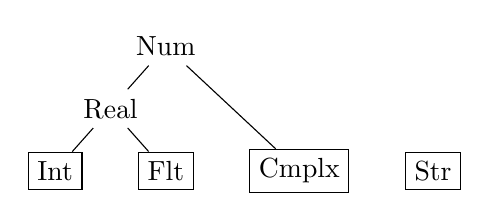
\begin{tikzpicture}[sibling distance=4em, level distance=2.25em,
	concrete/.style = {shape=rectangle, draw, align=center}]
	\node { Num }
	child { node { Real }
		child { node[concrete] { Int} }
		child { node[concrete] (NF) { Flt} } }
	child { node[concrete, right=2em of NF] (NC) {Cmplx} }
	;
	\node[concrete, right=2em of NC] {Str} ;
	\end{tikzpicture}
	\caption{\BetaJulia: type grammar and nominal hierarchy}
	\label{fig:bjsem-types}
\end{figure}

To simplify the development, we decided to work with particular 
nominal types and a hierarchy over them
(presented in~\figref{fig:bjsem-types} as a tree)
instead of a more abstract class table.
There are four concrete, leaf types (depicted in rectangles)
and two abstract types in the hierarchy. 
Formally, the hierarchy can be represented with a list of declarations
$\bjdeclsub{n_1}{n_2}$ read as ``$n_1$ is a declared subtype of $n_2$''
where $n ::= \cname \Alt \aname$.
In the case of \BetaJulia, the hierarchy is defined as follows:
\[
\NomH = [ \bjdeclsub{\tyreal}{\tynum}, 
\bjdeclsub{\tyint}{\tyreal}, \bjdeclsub{\tyflt}{\tyreal},
\bjdeclsub{\tycmplx}{\tynum} ].
\]
\TODO{requirements for hierarchy, like single parent, no cycles}

\subsection{Value Types}
%% -----------------------------------------------------------------------------

Not only concrete nominal types can be used as type tags
but also pair types. For example, \typair{\tyint}{\tyint}
or \typair{\tystr}{(\typair{\tyint}{\tyint})}.
Union types, on the other hand, cannot be type tags, 
as they potentially describe dissimilar values.
For instance, both integer and floating point values belong
to a union type \tyunion{\tyint}{\tyflt}.
Even type \tyunion{\tyint}{\tyint} is not a type tag, 
though it better be equivalent to a concrete type \tyint.

Types that can be used as type tags will be further referred to
as \defemph{value types}. 
Their formal definition is given in~\figref{fig:bjsem-value-types}:
value type $\vty \in \VType$ is either a concrete nominal type 
or a pair of value types. 
Note that $\VType \subset \Type$, i.e. each value type is a type.

\begin{figure}
	\[
	\begin{array}{rcl@{\qquad}l}
	\vty \in \VType & ::= & & \text{\emph{Value Types}}
	\\ &\Alt& \cname & \text{concrete nominal type}
	\\ &\Alt& \typair{\vty_1}{\vty_2} & \text{pair of value types}
	\end{array}
	\]
	\caption{Value types in \BetaJulia}
	\label{fig:bjsem-value-types}
\end{figure}


\subsection{Semantic Interpretation of Types}
%% -----------------------------------------------------------------------------

As mentioned earlier, the set of values represented by a value type \vty
is unambiguously characterized by~\vty itself
as long as each run-time value is tagged with a value type.
But what about an arbitrary type?

First, let us consider an abstract nominal type, e.g. \tynum. 
According to the nominal hierarchy, \tynum value 
is either a concrete complex number, or a real number, which, in turn,
is either a concrete integer or a floating point number.
Therefore, the set of values represented by \tynum 
is described by the set of value types $\{\tycmplx, \tyint, \tyflt\}$.

Next, pairs. Consider type \typair{\tystr}{\tyreal}:
each of its values is a pair of a string and a number. 
For example, \jlcode{("bread", 2)} and \jlcode{("milk", 2.75)} are such values, 
with type tags \typair{\tystr}{\tyint} and 
\typair{\tystr}{\tyflt}, respectively.

\begin{figure}
  \[
	\begin{array}{rcl}
	\interpty{\cdot}: \Type &\rightarrow& \PVType \\
	\interpty{\cname}  & = & \{\cname\} \\
	\interpty{\tyreal} & = & \{ \tyint, \tyflt \} \\
	\interpty{\tynum} & = & \{ \tyint, \tyflt, \tycmplx \} \\
	\interpty{\typair{\ty_1}{\ty_2}} & = & \{\typair{\vty_1}{\vty_2} 
	\Alt \vty_1 \in \interpty{\ty_1}, \vty_2 \in \interpty{\ty_2}\}\\
	\interpty{\tyunion{\ty_1}{\ty_2}} & = & 
	\interpty{\ty_1} \cup \interpty{\ty_2}
	\end{array}
  \]
%  	\interpty{\aname} & = & \{\cname\ \Alt \bjnomsub{\cname}{\aname} \} \\
%  (= \interpty{\tyreal} \cup \{\tycmplx\})
  \caption{Semantic Interpretation of \BetaJulia Types}
  \label{fig:bjsem-interpretation}
\end{figure}

Formally, the \emph{interpretation} of \BetaJulia types is defined
in~\figref{fig:bjsem-interpretation}.
Abstract types are interpreted according to the nominal hierarchy:
values of each abstract type are values of any of it value subtypes.
More generally, the interpretation of abstract types can be given in
then following way:
\[
\interpty{\aname} = \{\cname\ \Alt \bjnomsub{\cname}{\aname} \},
\]
where the relation $\bjnomsub{n_1}{n_2}$,
read ``$n_1$ is a nominal subtype of~$n_2$'',
is a transitive closure of $\bjdeclsub{n_1}{n_2}$:
\begin{mathpar}
	\inferrule*[right=]
	{ \bjdeclsub{n_1}{n_2} \in \NomH }
	{ \bjnomsub{n_1}{n_2} }
	
	\inferrule*[right=]
	{ \bjnomsub{n_1}{n_2} \\ \bjnomsub{n_2}{n_3} }
	{ \bjnomsub{n_1}{n_3} }.
\end{mathpar}
\TODO{Probably more on the semantic interpretation.}

Once we have the interpretation of types, we define \emph{semantic subtyping}
as the subset relation:
\[
\bjtruesemsub{\ty_1}{\ty_2} \quad \defsign \quad
\interpty{\ty_1} \subseteq \interpty{\ty_2}.
\]

%and the set of values represented by a type \ty can be characterized
%with the set of value types~$\vty_i$



\section{Syntactic Definitions of Subtyping}\label{sec:synsub}

The declarative subtyping is defined in~\figref{fig:bjsem-decl-sub}.
A big part of the definition is comprised of
the rules that are typically used to define syntactic subtyping 
in languages with base types, unions, and pairs.
Namely, reflexivity and transitivity (\RD{Refl} and \RD{Trans}), 
subtyping of pairs (\RD{Pairs}),
and subtyping of unions (\RD{UnionL}, \RD{UnionR1}, \RD{UnionR2}).
Though \RD{UnionR*} rules are seemingly very strict, 
transitivity allows us to derive judgments such as
$\bjsub{\tyint}{\tyunion{\tystr}{\tyreal}}$ via
$\bjsub{\tyint}{\tyreal}$ and $\bjsub{\tyreal}{\tyunion{\tystr}{\tyreal}}$.
Note that we do need the syntactic definition of subtyping
to be \emph{reflexive} and \emph{transitive}
because so is the semantic subtyping (due to the subset relation).

Semantic subtyping also forces us to add rules 
for distributing pairs over unions, \RD{Distr1} and \RD{Distr2}. 
The reason is that types such as 
\tyunion{(\typair{\tystr}{\tyint})}{(\typair{\tystr}{\tyflt})}
and \typair{\tystr}{(\tyunion{\tyint}{\tyflt})} 
have the same semantic interpretation 
$\{\typair{\tystr}{\tyint}, \typair{\tystr}{\tyflt}\}$.
Therefore, the types need to be equivalent within the declarative definition,
i.e., subtyping between them should hold in both directions.
One direction is trivial:
\begin{mathpar}{\small
\inferrule*[right=]
{ \inferrule*[right=]
  { \bjsub{\tystr}{\tystr} \\ \bjsub{\tyint}{\tyunion{\tyint}{\tyflt}} }
  { \bjsub{\typair{\tystr}{\tyint}}
  	  {\typair{\tystr}{(\tyunion{\tyint}{\tyflt})}} } \\
  \inferrule*[right=]
  { \ldots }
  { \bjsub{\typair{\tystr}{\tyflt}}
  	  {\ldots} } }
{ \bjsub{\tyunion{(\typair{\tystr}{\tyint})}{(\typair{\tystr}{\tyflt})}}
	{\typair{\tystr}{(\tyunion{\tyint}{\tyflt})}} }.
}\end{mathpar}
But the other direction,  
\[
\bjsub{\typair{\tystr}{(\tyunion{\tyint}{\tyflt})}}
  {\tyunion{(\typair{\tystr}{\tyint})}{(\typair{\tystr}{\tyflt})}},
\]
cannot be derived without \RD{Distr2} rule: 
\typair{\tystr}{(\tyunion{\tyint}{\tyflt})} is 
not a subtype of either \typair{\tystr}{\tyint} or \typair{\tystr}{\tyflt},
so we cannot apply \RD{UnionR*} rules\footnote{Transitivity
  does not help in this case.}.

Finally, let us look at subtyping of nominal types.
There are four obvious rules coming directly 
from the nominal hierarchy, for instance, \RD{RealNum} mirrors the fact 
that $\bjdeclsub{\tyreal}{\tynum} \in \NomH$.
Using these rules, judgments such as $\bjsub{\tyint}{\tynum}$ 
can be derived by transitivity.
The most interesting rules in the system are
\RD{RealUnion} and \RD{NumUnion} (\colorbox{light-gray}{highlighted}
in~\figref{fig:bjsem-decl-sub})~--- they are dictated by semantic subtyping
similarly to the distributivity rules.
Namely, we need them to achieve equivalence
between, e.g., types \tyunion{\tyint}{\tyflt} and \tyreal, 
which have the same interpretation $\{\tyint, \tyflt\}$.

%Before we define an inductive declarative relation $\bjsub{\ty_1}{\ty_2}$.

%Besides, the ability to reason about types directly,
%without appealing to all their value subtypes.
%Therefore, we provide  definitions of subtyping
%in the form of inductive rule

\begin{figure}
	\begin{mathpar}
		\inferrule*[right=SD-Refl]
		{ }
		{ \bjsub{\ty}{\ty} }
		
		\inferrule*[right=SD-Trans]
		{ \bjsub{\ty_1}{\ty_2} \\ \bjsub{\ty_2}{\ty_3} }
		{ \bjsub{\ty_1}{\ty_3} }		
		\\
		
		\inferrule[SD-IntReal]
		{ }
		{ \bjsub{\tyint}{\tyreal} }
		
		\inferrule[SD-FltReal]
		{ }
		{ \bjsub{\tyflt}{\tyreal} }
		\\
		
		\inferrule[{SD-RealNum}]
		{ }
		{ \bjsub{\tyreal}{\tynum} }
	
		\inferrule[{SD-CmplxNum}]
		{ }
		{ \bjsub{\tycmplx}{\tynum} }
		\\
		
		\colorbox{light-gray}{$
		\inferrule[SD-RealUnion]
		{ }
		{ \bjsub{\tyreal}{\tyunion{\tyint}{\tyflt}} }
		$}
		
		\colorbox{light-gray}{$
		\inferrule[SD-NumUnion]
		{ }
		{ \bjsub{\tynum}{\tyunion{\tyreal}{\tycmplx}} }
		$}
		\\
		
		\inferrule*[right=SD-Pair]
		{ \bjsub{\ty_1}{\ty'_1} \\ \bjsub{\ty_2}{\ty'_2} }
		{ \bjsub{\typair{\ty_1}{\ty_2}}{\typair{\ty'_1}{\ty'_2}} }
		\\
		
		\inferrule*[right=SD-UnionL]
		{ \bjsub{\ty_1}{\ty'} \\ \bjsub{\ty_2}{\ty'} }
		{ \bjsub{\tyunion{\ty_1}{\ty_2}}{\ty'} }
		\\
		
		\inferrule[{SD-UnionR1}]
		{ }
		{ \bjsub{\ty_1}{\tyunion{\ty_1}{\ty_2}} }
		
		\inferrule[{SD-UnionR2}]
		{ }
		{ \bjsub{\ty_2}{\tyunion{\ty_1}{\ty_2}} }
		\\
		
		\inferrule*[right=SD-Distr1]
		{ }
		{ \bjsub{\typair{(\tyunion{\ty_{11}}{\ty_{12}})}{\ty_2}}
			{\tyunion{(\typair{\ty_{11}}{\ty_2})}{(\typair{\ty_{12}}{\ty_2})}} }
		
		\inferrule*[right=SD-Distr2]
		{ }
		{ \bjsub{\typair{\ty_1}{(\tyunion{\ty_{21}}{\ty_{22}})}}
			{\tyunion{(\typair{\ty_1}{\ty_{21}})}{(\typair{\ty_1}{\ty_{22}})}} }
	\end{mathpar}
	\caption{Declarative Subtyping for \BetaJulia}
	\label{fig:bjsem-decl-sub}
\end{figure}


\subsection{Correctness of Declarative Subtyping}
%% -----------------------------------------------------------------------------

In order to show that the declarative syntactic subtyping is correct
with respect to the semantic subtyping,
we need to prove that the former is sound and complete with respect
to the latter one, that is:
\[
\forall \ty_1, \ty_2.\ (\bjsub{\ty_1}{\ty_2} \iff \bjtruesemsub{\ty_1}{\ty_2}).
\]
As discussed in~\secref{sec:syn-model-of-semsub}, there is 
a sound and complete syntactic model of semantic subtyping,
$\bjsemsub{\ty_1}{\ty_2}$.
So for proofs, we will be using the model:
%, based on the straightforward matching relation.
\begin{equation}\label{eq:declsub-eq-semsub}
\forall \ty_1, \ty_2.\ (\bjsub{\ty_1}{\ty_2} \iff \bjsemsub{\ty_1}{\ty_2}).
\end{equation}

\begin{figure}
  \[
	\begin{array}{rcl}
	\NF: \Type &\rightarrow& \Type \\
	\NF(\cname) &=& \cname \\
	\colorbox{light-gray}{\NF(\tyreal)} &=&
	\colorbox{light-gray}{\tyunion{\tyint}{\tyflt}} \\
	\colorbox{light-gray}{\NF(\tynum)} &=&
	\colorbox{light-gray}{\tyunion{\tyunion{\tyint}{\tyflt}}{\tycmplx}} \\
	\NF(\typair{\ty_1}{\ty_2}) &=& \unprs(\NF(\ty_1), \, \NF(\ty_2))	\\
	\NF(\tyunion{\ty_1}{\ty_2}) &=& \tyunion{\NF(\ty_1)}{\NF(\ty_2)} \\
	\end{array}
  \]
	\caption{Computing Normal Form of Types in \BetaJulia}
	\label{fig:bjsem-calc-nf}
\end{figure}


\subsection{Reductive Subtyping}\label{sec:redsub}
%% -----------------------------------------------------------------------------

The declarative definition is not syntax-directed
and cannot be directly turned into a subtyping algorithm.
For one, the transitivity rule \RD{Trans} 
overlaps with any other rule in the system
and also requires ``coming up'' with an intermediate type $\ty_2$
to conclude $\bjsub{\ty_1}{\ty_3}$.
For instance, to derive %in order
\[\bjsub{\typair{\tystr}{\tyreal}}
{(\typair{\tystr}{\tyint}) \cup (\typair{\tystr}{\tystr}) 
	\cup (\typair{\tystr}{\tyflt})},\]
we need to apply transitivity several times, in particular, 
with the intermediate type $\typair{\tystr}{(\tyunion{\tyint}{\tyflt})}$.
Another source of overlap is the reflexivity and distributivity rules.
%Another issue is that the rules \RD{Refl}, \RD{UnionR*}, and \RD{Distr*}
%require deep structural comparison of the left- and right-hand side types.
%For example, in order for \RD{UnionR1} to be applicable to some 
%$\bjsub{\ty_a}{\ty_b}$, not only $\ty_b$ must be a union, 
%but also its left component should be equal to $\ty_a$.

\begin{figure}
	\begin{mathpar}
		\colorbox{light-gray}{$
		\inferrule*[right=SR-BaseRefl]
		{ }
		{ \bjsubr{\cname}{\cname} }
		$}
		\\
		
		\inferrule[SR-IntReal]
		{ }
		{ \bjsubr{\tyint}{\tyreal} }
		
		\inferrule[SR-FltReal]
		{ }
		{ \bjsubr{\tyflt}{\tyreal} }
		\\
	
		\inferrule[SR-CmplxNum]
		{ }
		{ \bjsubr{\tycmplx}{\tynum} }
		
		\colorbox{light-gray}{$
		\inferrule[SR-IntNum]
		{ }
		{ \bjsubr{\tyint}{\tynum} }
		$}
		
		\colorbox{light-gray}{$
		\inferrule[SR-FltNum]
		{ }
		{ \bjsubr{\tyflt}{\tynum} }
		$}
		\\
		
		\inferrule*[right=SR-Pair]
		{ \bjsubr{\ty_1}{\ty'_1} \\ \bjsubr{\ty_2}{\ty'_2} }
		{ \bjsubr{\typair{\ty_1}{\ty_2}}{\typair{\ty'_1}{\ty'_2}} }
		\\
		
		\inferrule*[right=SR-UnionL]
		{ \bjsubr{\ty_1}{\ty'} \\ \bjsubr{\ty_2}{\ty'} }
		{ \bjsubr{\tyunion{\ty_1}{\ty_2}}{\ty'} }
		\\
		
		\colorbox{light-gray}{$
		\inferrule[SR-UnionR1]
		{ \bjsubr{\ty}{\ty'_1} }
		{ \bjsubr{\ty}{\tyunion{\ty'_1}{\ty'_2}} }
		$}
		
		\colorbox{light-gray}{$
		\inferrule[SR-UnionR2]
		{ \bjsubr{\ty}{\ty'_2} }
		{ \bjsubr{\ty}{\tyunion{\ty'_1}{\ty'_2}} }
		$}
		\\
		
		\colorbox{light-gray}{$
		\inferrule*[right=SR-NF]
		{ \bjsubr{\NF(\ty)}{\ty'} }
		{ \bjsubr{\ty}{\ty'} }
		$}
	\end{mathpar}
	\caption{Reductive subtyping for \BetaJulia}
	\label{fig:bjsem-red-sub}
\end{figure}

%The syntax-directed reductive definition\footnote{The definition
%	%the rules can be easily turned 
%	%into a subtyping algorithm.
%	is not deterministic, though.	For example, there are two ways to derive 
%	$\bjsubr{\typair{\tystr}{(\tyunion{\tyint}{\tyflt})}}
%	{\typair{\tystr}{(\tyunion{\tyint}{\tyflt})}}$: 
%	either by immediately applying \RR{Pair}, 
%	or by first normalizing the left-hand side with \RR{NF}.} of subtyping
%is presented in~\figref{fig:bjsem-red-sub}.
By contrast, the rules of reductive subtyping enable
straightforward bottom-to-top reasoning;
the rules are presented in~\figref{fig:bjsem-red-sub}.
The reductive definition lacks the most problematic rules
of declarative subtyping, 
i.e. general reflexivity, transitivity, and distributivity.
Some of the inductive rules have the exact declarative counterparts,
e.g. subtyping of pairs (\RR{Pair}) or
subtyping of a union on the left (\RR{UnionL}).
%for instance, the rule for subtyping of pairs (\RR{Pair}) 
%or the rule for a union on the left (\RR{UnionL}).

The differing rules are \colorbox{light-gray}{highlighted}.
The explicit reflexivity rule \RR{BaseRefl} now only works with 
concrete nominal types, which is enough 
for the reductive definition to be reflexive.
The definition also has to be transitive,
so the effects of using transitivity get incorporated into
other rules, such as subtyping of nominal types (\RR{IntNum}, \RR{FltNum})
or subtyping of a union on the right (\RR{UnionR1}, \RR{UnionR2}).

The last rule of the definition, \RR{NF}, is the most important,
as it covers all useful interactions of transitivity and distributivity 
that are possible in the declarative definition.
The rule rewrites type \ty into its \defemph{normal form} $\NF(\ty)$
before applying other subtyping rules.
%This covers all useful applications of transitivity and distributivity 
%that are possible in the declarative definition.
The normalized type has the form $\vty_1 \cup \vty_2 \cup \ldots \cup \vty_n$,
i.e. a union of value types
(we omit parenthesis because union is associative).
The normalization function $\NF$ is presented in~\figref{fig:bjsem-calc-nf}
(the auxiliary function $\unprs$ 
can be found in~\figref{fig:bjsem-calc-nf-full}, \appref{app:nf}).
It produces a type in \emph{disjunctive normal form}
by replacing an abstract nominal type 
with the union of all its concrete subtypes, 
and a pair of unions with the union of pairs of value types
(each of this pairs is itself a value type),
for instance:
\[
\NF(\typair{\tystr}{(\tyunion{\tyint}{\tyflt})}) =
\tyunion{(\typair{\tystr}{\tyint})}{(\typair{\tystr}{\tyflt})}.
\]
As we show in~\secref{sec:declsub-correct}, a type and its normal form are
equivalent in the declarative definition.
This property is essential for reductive subtyping 
being equivalent to declarative one.
%an essential property
%for reductive subtyping being equivalent to declarative one.

\begin{figure}
  \[
	\begin{array}{rcl}
	\NF: \Type &\rightarrow& \Type \\
	\NF(\cname) &=& \cname \\
	\colorbox{light-gray}{\NF(\tyreal)} &=&
	\colorbox{light-gray}{\tyunion{\tyint}{\tyflt}} \\
	\colorbox{light-gray}{\NF(\tynum)} &=&
	\colorbox{light-gray}{\tyunion{\tyunion{\tyint}{\tyflt}}{\tycmplx}} \\
	\NF(\typair{\ty_1}{\ty_2}) &=& \unprs(\NF(\ty_1), \, \NF(\ty_2))	\\
	\NF(\tyunion{\ty_1}{\ty_2}) &=& \tyunion{\NF(\ty_1)}{\NF(\ty_2)} \\
	\end{array}
  \]
	\caption{Computing normal form of \BetaJulia types}
	\label{fig:bjsem-calc-nf}
\end{figure}

\paragraph{Subtyping Algorithm.}
Though the reductive rules are not syntax-directed per se,
if a derivation of $\bjsub{\ty}{\ty'}$ exists,
it can always be found by the following algorithm:
(1) apply the normalization rule \RR{NF} once, i.e. normalize $\ty$;
(2) use all the other (syntax-directed) rules to build the derivation of
$\bjsub{\NF(\ty)}{\ty'}$ in the usual manner, bottom to top.

However, this algorithm does not always produce the shortest derivation.
For instance, for
$\bjsubr{\typair{\tystr}{(\tyunion{\tyint}{\tyflt})}}
	    {\typair{\tystr}{\tyreal}}$,
it produces a derivation with eight applications of the rules, 
whereas the shortest derivation needs only five applications
(see~\appref{app:example-deriv}).
It is possible that in practice, an algorithm that tries the short path first 
and only then resorts to normalization would work better.

The actual Julia implementation uses a clever algorithm 
to check subtyping of tuples and unions 
without having to normalize types~\cite{bib:Chung19}.
The algorithm is equivalent to the normalization based one discussed above,
but instead of computing the whole normal form, 
it computes only the components of the normalized type, one at a time.

Note that the rules for subtyping of nominal types do not have to be built-in.
Instead of five separate rules, as presented in~\figref{fig:bjsem-red-sub},
we can use a single rule that relies on the relation 
$\bjnomsub{n_1}{n_2}$ ($n_1$ transitively extends $n_2$)
from~\secref{subsec:interp}:
\begin{mathpar}
	\inferrule*[right=SR-Nom]
	{ \bjnomsub{n_1}{n_2} }
	{ \bjsub{n_1}{n_2} }.
\end{mathpar}
Then, for any $n_1$ and $n_2$, the relation $\bjnomsub{n_1}{n_2}$ 
can be checked algorithmically, using the nominal hierarchy $\NomH$.


% for using the normal form (\RR{NF}).
%Note that the last rule also takes care of distributivity.

%With the reductive subtyping, the example above can be derived as follows:
%\begin{mathpar}\small
%\inferrule*[right=]
%{ \inferrule*[right=]
%  { \bjsub{\typair{\tystr}{\tyint}}{(\typair{\tystr}{\tyint}) \ldots} \\
%    \bjsub{\typair{\tystr}{\tyflt}}{\ldots (\typair{\tystr}{\tyflt})}  }	
%  { \bjsub{\tyunion{(\typair{\tystr}{\tyint})}{(\typair{\tystr}{\tyflt})}}
%	{(\typair{\tystr}{\tyint}) \cup \ldots \cup (\typair{\tystr}{\tyflt})} } }
%{ \bjsub{\typair{\tystr}{\tyreal}}
%	{(\typair{\tystr}{\tyint}) \cup (\typair{\tystr}{\tystr}) 
%		\cup (\typair{\tystr}{\tyflt})} }.
%\end{mathpar}
%In the very bottom, we use \RR{NF}, and then \RR{UnionL} in the level above.
%To complete the top of derivation, we would also need to use \RR{UnionR*}, 
%\RR{Pair}, and \RR{BaseRefl}.




\section{Properties of Subtyping Relations}\label{sec:proofs}

\subsection{Correctness of Declarative Subtyping}\label{sec:declsub-correct}
%% -----------------------------------------------------------------------------

\begin{figure}
	\begin{mathpar}
		\inferrule*[right=MT-CName]
		{ }
		{ \bjmtch{\cname}{\cname} }		
		\\
		
		\inferrule[MT-IntReal]
		{ }
		{ \bjmtch{\tyint}{\tyreal} }
		
		\inferrule[MT-FltReal]
		{ }
		{ \bjmtch{\tyflt}{\tyreal} }
		\\
		
		\inferrule[MT-IntNum]
		{ }
		{ \bjmtch{\tyint}{\tynum} }
		
		\inferrule[MT-FltNum]
		{ }
		{ \bjmtch{\tyflt}{\tynum} }
		
		\inferrule[MT-CmplxNum]
		{ }
		{ \bjmtch{\tycmplx}{\tynum} }
		\\
		
		\inferrule*[right=MT-Pair]
		{ \bjmtch{\vty_1}{\ty_1} \\ \bjmtch{\vty_2}{\ty_2} }
		{ \bjmtch{\typair{\vty_1}{\vty_2}}{\typair{\ty_1}{\ty_2}} }
		\\
		
		\inferrule*[right=MT-Union1]
		{ \bjmtch{\vty}{\ty_1}  }
		{ \bjmtch{\vty}{\tyunion{\ty_1}{\ty_2}} }
		
		\inferrule*[right=MT-Union2]
		{ \bjmtch{\vty}{\ty_2}  }
		{ \bjmtch{\vty}{\tyunion{\ty_1}{\ty_2}} }
	\end{mathpar}
	\caption{Matching relation in \BetaJulia}
	\label{fig:bjsem-match}
\end{figure}

In order to show that the declarative definition of subtyping 
is equivalent to the semantic definition,
we need to prove that the former is sound and complete with respect
to the latter, that is:
\begin{equation}\label{eq:declsub-correct-truesemsub}
\forall \ty_1, \ty_2.\ (\bjsub{\ty_1}{\ty_2} \iff \bjtruesemsub{\ty_1}{\ty_2}).
\end{equation}

We find that instead of directly proving~\eqref{eq:declsub-correct-truesemsub},
it is more convenient to show that declarative subtyping
is equivalent to the following relation,
referred to as \defemph{matching-based semantic subtyping}:
\begin{equation}\label{eq:semsub-def}
\bjsemsub{\ty_1}{\ty_2} \quad \defsign \quad
\forall \vty.\ (\bjmtch{\vty}{\ty_1} \implies\ \bjmtch{\vty}{\ty_2}).
\end{equation}
The definition~\eqref{eq:semsub-def}
relies on the relation $\bjmtch{\vty}{\ty}$ 
(defined in~\figref{fig:bjsem-match}), read ``tag~\vty matches type~\ty'', 
which we call the \defemph{matching relation}.

Tag-based and matching-based semantic subtyping relations 
are equivalent:
%\begin{equation}
\[
\forall \ty_1, \ty_2.\ 
(\bjsemsub{\ty_1}{\ty_2} \iff \bjtruesemsub{\ty_1}{\ty_2}).
\]
%\end{equation}
To see why, recall that tag-based semantic subtyping~\eqref{eq:truesemsub-def} 
is defined as $\interpty{\ty_1} \subseteq \interpty{\ty_2}$
and the subset relation $X \subseteq Y$ as
$\forall x.\ (x \in X \implies x \in Y)$.
Therefore, the definition~\eqref{eq:truesemsub-def} can be 
rewritten as:
\begin{equation}\label{eq:truesemsub-def-new}
\bjtruesemsub{\ty_1}{\ty_2} \;\defsign \;
%\interpty{\ty_1} \subseteq \interpty{\ty_2} \; \defsign \;
\forall \vty.\ (\vty \in \interpty{\ty_1} \implies \vty \in \interpty{\ty_2}).
\end{equation}
It is easy to show by induction on \ty that the matching relation
is equivalent to the belongs-to relation $\vty \in \interpty{\ty}$. 
Therefore, the definitions~\eqref{eq:semsub-def}
and~\eqref{eq:truesemsub-def-new} are also equivalent.

Since $\bjtruesemsub{\ty_1}{\ty_2}$ is equivalent to $\bjsemsub{\ty_1}{\ty_2}$
and the equivalence relation $\iff$ is transitive,
to show~\eqref{eq:declsub-correct-truesemsub},
it suffices to prove the following theorem.

\begin{theorem}[Correctness of Declarative Subtyping]\label{thm:declsub-correct}
	\[
	\forall \ty_1, \ty_2.\ (\bjsub{\ty_1}{\ty_2} \iff\ \bjsemsub{\ty_1}{\ty_2})
	\]
\end{theorem}

The full proof of~\thmref{thm:declsub-correct} is 
Coq-mechanized~\cite{bib:MiniJlCoq},
so here, we only discuss some key aspects.
First of all, subtyping a value type coincides with matching the value type:
\begin{equation}\label{eq:mtch-eq-declsub}
\forall \vty, \ty.\ (\bjsub{\vty}{\ty} \iff\ \bjmtch{\vty}{\ty}).
\end{equation}
Having that, we can prove 
$\bjsub{\ty_1}{\ty_2} \implies \bjsemsub{\ty_1}{\ty_2}$,
i.e. the soundness direction of~\thmref{thm:declsub-correct}
(below, we embed the definition~\eqref{eq:semsub-def} of 
matching-based semantic subtyping):
\begin{equation}\label{eq:declsub-imp-semsub}
\forall \ty_1, \ty_2.\ 
(\bjsub{\ty_1}{\ty_2} \implies\ 
\forall \vty.\ [\bjmtch{\vty}{\ty_1} \implies\ \bjmtch{\vty}{\ty_2}]).
\end{equation}
Knowing $\bjsub{\ty_1}{\ty_2}$ and $\bjmtch{\vty}{\ty_1}$,
we need to show that $\bjmtch{\vty}{\ty_2}$.
First, by applying~\eqref{eq:mtch-eq-declsub} to $\bjmtch{\vty}{\ty_1}$,
we get $\bjsub{\vty}{\ty_1}$.
Then, $\bjsub{\vty}{\ty_2}$ follows from $\bjsub{\vty}{\ty_1}$ 
and $\bjsub{\ty_1}{\ty_2}$ by transitivity.
Finally, by applying~\eqref{eq:mtch-eq-declsub} again,
we get $\bjmtch{\vty}{\ty_2}$. \qed

The other direction of~\thmref{thm:declsub-correct} is more challenging: 
\begin{equation}\label{eq:declsub-complete}
\forall \ty_1, \ty_2.\ 
(\bjsemsub{\ty_1}{\ty_2} \implies\ \bjsub{\ty_1}{\ty_2}).
\end{equation}
The key observation here is that~\eqref{eq:declsub-complete} can be shown 
for $\ty_1$ in \emph{normal form},
i.e. $\ty_1 \equiv \vty_1 \cup \vty_2 \cup \ldots \cup \vty_n$
(formally, this fact is denoted by predicate $\InNF(\ty_1)$ 
defined in~\figref{fig:bjsem-innf}, \appref{app:nf}):
\begin{equation}\label{eq:nf-declsub-complete}
\forall \ty_1, \ty_2 \Alt \InNF(\ty_1).\
(\bjsemsub{\ty_1}{\ty_2} \implies\ \bjsub{\ty_1}{\ty_2}).
\end{equation}
In this case, in the definition~\eqref{eq:semsub-def}
of $\bjsemsub{\ty_1}{\ty_2}$, the only
value types $\vty$ that match $\ty_1$ and $\ty_2$ are $\vty_i$ of $\ty_1$. 
By~\eqref{eq:mtch-eq-declsub}, we know that matching implies subtyping,
so we have that all $\bjsub{\vty_i}{\ty_2}$.
From the latter, it is easy to show that 
$\bjsub{(\vty_1 \cup \vty_2 \cup \ldots \cup \vty_n)}{\ty_2}$ because,
according to the \RD{UnionL} rule,
subtyping of the left-hand side union amounts to subtyping its components.
In addition to~\eqref{eq:nf-declsub-complete}, we need several more facts.
\begin{itemize}
  \item Function $\NF$ produces a type in normal form:
	\begin{equation}\label{eq:nf-innf}
	\forall \ty.\ \InNF(\NF(\ty)).
	\end{equation}
  \item Normalized type is equivalent to the source type:
    \begin{equation}\label{eq:nf-declsub-eq}
    \forall \ty.\;\ \bjsub{\NF(\ty)}{\ty}\ \land\ \bjsub{\ty}{\NF(\ty)}.
    \end{equation}
  \item Normalization preserves subtyping relation:
    \begin{equation}\label{eq:nf-semsub}
    \forall \ty_1, \ty_2.\ 
    (\bjsemsub{\ty_1}{\ty_2} \implies\ \bjsemsub{\NF(\ty_1)}{\ty_2}).
    \end{equation}
\end{itemize}
To prove~\eqref{eq:declsub-complete}, we need to show $\bjsub{\ty_1}{\ty_2}$
given $\bjsemsub{\ty_1}{\ty_2}$. 
For this, we first apply~\eqref{eq:nf-semsub} to $\bjsemsub{\ty_1}{\ty_2}$,
which gives $\bjsemsub{\NF(\ty_1)}{\ty_2}$. 
Then we can apply~\eqref{eq:nf-declsub-complete} to the latter
because of~\eqref{eq:nf-innf} to get $\bjsub{\NF(\ty_1)}{\ty_2}$.
Finally, \eqref{eq:nf-declsub-eq} and transitivity 
gives $\bjsub{\ty_1}{\ty_2}$. \qed

\subsection{Reductive Subtyping}\label{sec:redsub-correct}
%% -----------------------------------------------------------------------------

Since we have already shown that declarative subtyping is
equivalent to semantic subtyping, it suffices to show that
reductive subtyping is equivalent to declarative one:

\begin{theorem}[Correctness of Reductive Subtyping]\label{thm:redsub-correct}
\[
\forall \ty_1, \ty_2.\ (\bjsubr{\ty_1}{\ty_2} \iff\ \bjsub{\ty_1}{\ty_2})
\]
\end{theorem}

The proof is split into two parts: soundness and completeness.
For soundness (completeness), 
by induction on $\bjsubr{\ty_1}{\ty_2}$ ($\bjsub{\ty_1}{\ty_2}$),
we show that for each \RR{}\!rule (\RD{}\!rule) it is possible to build
a corresponding declarative (reductive) derivation 
using \RD{}\!rules (\RR{}\!rules).

The soundness direction is mostly straightforward, as most \RR{}\!rules
have an immediate \RD{}\!counterpart (or require one extra application
of transitivity).
In the case of \RR{NF}, the induction hypothesis of the proof,
$\bjsub{\NF(\ty_1)}{\ty_2}$, 
and the fact that $\bjsub{\ty_1}{\NF(\ty_1)}$~\eqref{eq:nf-declsub-eq}
allow to conclude $\bjsub{\ty_1}{\ty_2}$.

The challenging part of the proof is to show completeness,
as this requires proving that the reductive definition 
is \emph{reflexive}, \emph{transitive}, and \emph{distributive}
(\appref{app:proofs}).

%To prove transitivity and distributivity, 
%we need several auxiliary statements:
%\begin{enumerate}
%  \item $\bjsubr{\ty}{\ty'}\ \implies\ \bjsubr{\NF(\ty)}{\ty'}$,
%  \item $\bjsubr{\NF(\ty_1)}{\NF(\ty_2)}\;\;\ \land\;\; \bjsubr{\NF(\ty_2)}{\ty_3}$\\
%     $\implies \bjsubr{\NF(\ty_1)}{\ty_3}$,
%  \item $\bjsubr{\NF(\ty)}{\NF(\ty')}\ \implies\ \bjsubr{\ty}{\ty'}$.
%\end{enumerate}
%Having all the facts, we can prove completeness by induction
%on a derivation of $\bjsub{\NF(\ty_1)}{\ty_2}$.
%For details, the reader can refer to the full Coq-proof.

\begin{theorem}[Decidability of Reductive Subtyping]\label{thm:redsub-decidable}
\[
\forall \ty_1, \ty_2.\ 
(\bjsubr{\ty_1}{\ty_2}\quad \lor\quad \lnot [\bjsubr{\ty_1}{\ty_2}])
\]
\end{theorem}

To prove the theorem, 
it suffices to show that reductive subtyping is decidable
when $\ty_1$ is in normal form.
This is done by induction on a derivation of $\InNF(\ty_1)$.
We refer the reader to \appref{app:proofs} for more details.

% By induction on a derivation of $\InNF(\ty_1)$, we can show
% that the reductive subtyping is decidable for $\ty_1 | \InNF(\ty_1)$.
% In this case, $\ty_1$ is either a value type or a union of normalized types.
% If it is a value type, subtyping is equivalent to matching,
% and matching is decidable.
% If $\ty_1$ is a union $\tyunion{\ty_a}{\ty_b}$, 
% we use induction hypothesis for components and the fact that
% subtyping union on the left-hand side
% $\bjsubr{\tyunion{\ty_a}{\ty_b}}{\ty'}$ implies $\bjsubr{\ty_a}{\ty'}$
% and $\bjsubr{\ty_b}{\ty'}$.
% Since $\InNF(\NF(\ty_1))$, we can use the decidability 
% of $\bjsubr{\NF(\ty_1)}{\ty_2}$ to prove decidability
% of $\bjsubr{\ty_1}{\ty_2}$.


\section{Semantic Subtyping and\\ Multiple Dynamic Dispatch}
\label{sec:discussion}

In this section, we describe in more details how subtyping
can be used to implement multiple dynamic dispatch,
and also discuss why using the semantic subtyping for this
might not be a good idea.

As an example, consider the following methods\footnote{In the context of MDD, 
	different implementations of 
	the same function are usually called \emph{methods},
	and the set of all methods is called a \emph{generic function}.}
of the addition function (we assume that function \jlcode{flt} 
converts its argument to a float):
\begin{lstminijl}
+(x::Int, y::Int) = prim_add_int(x, y) 
+(x::Flt, y::Flt) = prim_add_flt(x, y) 
+(x::Int%*$\cup$*)Flt, y::Int%*$\cup$*)Flt) = prim_add_flt(flt(x), ..)
\end{lstminijl}
and the function call \jlcode{3 + 5}.
How exactly does dispatch work?

One approach, adopted, for example, 
by the Julia language~\cite{Bezanson2015AbstractionIT}, 
is to use subtyping on tuples~\cite{bib:Leavens:1998:mddtuples}.
Namely, method signatures and function calls are interpreted as tuple types,
and then subtyping is used to determine applicable methods 
as well as pick one of them.
In the example above, the three methods are interpreted 
as the following types (from top to bottom):\\
\jlcode{mII $\equiv$ Int $\times$ Int}\\
\jlcode{mFF $\equiv$ Flt $\times$ Flt}\\
\jlcode{mUU $\equiv$ (Int$\cup$Flt) $\times$ (Int$\cup$Flt)}\\
and the call~--- as type \jlcode{cII $\equiv$ Int $\times$ Int}.
To resolve the call, language run-time ought to perform two steps.
\begin{enumerate}
  \item Find applicable methods (if any). For this, we check subtyping between
    the type of the call, \jlcode{cII}, and the method signatures.
    Since \jlcode{cII $<:$ mII} and \jlcode{cII $<:$ mUU} but
    \jlcode{cII $\not{<:}$ mFF}, only two methods are applicable,
    \jlcode{mII} for integers and \jlcode{mUU} for mixed-type numbers.
  \item Pick the best, most specific of the applicable methods
    (if there is one).
    For this, we check subtyping relation between all applicable methods.
    In this example, naturally, we would like \jlcode{mII} to be called
    for addition of integers. And indeed, since \jlcode{mII $<:$ mUU},
    the integer addition is considered the most specific.
\end{enumerate}
Let us also consider the call \jlcode{3.14 + 5}. Its type is
\jlcode{Int $\times$ Flt}, and there is only one applicable method that is
a supertype of the call type~--- \jlcode{mUU}, so it should be called.

Is is important to understand what happens if the programmer defines
several implementations with the same argument types. 
In the case of a static language, an error can be reported.
In the case of a dynamic language, however, the second implementation
simply replaces the earlier one, in the same way as an assignment
to a variable replaces its previous value.

For instance, consider a program 
that contains the three implementations of \jlcode{(+)} from above
and also the following:
\begin{lstminijl}
+(x::Real, y::Real) = ...   # mRR
print(3.14 + 5)	 
\end{lstminijl}
According to the semantic subtyping, type \jltype{Real} is equivalent
to \jltype{Int$\cup$Flt} in \BetaJulia. 
Therefore, implementation of \jlcode{mRR} will replace \jlcode{mUU}, 
and the call \jlcode{3.14 + 5} will be dispatched to \jlcode{mRR}.

Unfortunately, the semantics of the program above is not stable.
If the programmer adds a new type into the nominal hierarchy,
e.g. \jlcode{Int8 $<:$ Real}, type \jlcode{Real} is not
equivalent to \jltype{Int$\cup$Flt} anymore.
Therefore, if we run the program again, types of \jlcode{mUU} and \jlcode{mRR}
will be different, and so the implementation of \jlcode{mRR} 
will not replace \jlcode{mUU}. 
Since \jlcode{mUU $<:$ mRR}, the call \jlcode{3.14 + 5} 
will be dispatched to \jlcode{mUU}, not \jlcode{mRR} as before.

We can gain stability by removing the rules that 
equate abstract nominal types with the union of their subtypes,
i.e., \RD{RealUnion} and \RD{NumUnion} in the declarative definition.\footnote{
    To get an equivalent reductive subtyping, we need to change 
    the \RR{NF} rule: replace normalization function $\NF$ with $\NFAt$ 
    (\figref{fig:bjnom-calc-nf-full}, \appref{app:nf}).}
To fix the discrepancy between this definition and the semantic interpretation,
we can change the latter by accounting for ``future nominal types'',
e.g. $\interpty{\tyreal} = \{\tyint, \tyflt, X\}$.
It needs to be understood whether such an interpretation provides us with
a useful intuition about subtyping.


%MDD allows to have several implementations of the same function,
%with the best implementation for a particular call being picked 
%at run-time based on the types of the arguments.
%As an example, consider two implementations of shape intersection
%(implementations are usually called \emph{methods}):
%\begin{verbatim}
%intersect(r1::Rectangle, r2::Rectangle) = ...
%intersect(s1::Shape, s2::Shape) = ...
%\end{verbatim}
%and two function calls, \jlcode{intersect(Circle(..), Circle(..))}
%and \jlcode{intersect(Rectangle(..), Rectangle(..))},
%assuming that \jltype{Circle} is a subtype of \jltype{Shape}.
%The method signatures can be interpreted as tuple types
%\jltype{mRR $\equiv$ Rectangle $\times$ Rectangle} 
%and \jltype{mSS $\equiv$ Shape $\times$ Shape},
%and the function calls~--- as tuple types 
%\jltype{CC $\equiv$ Circle $\times$ Circle} 
%and \jltype{RR $\equiv$ Rectangle $\times$ Rectangle}.
%To resolve the calls, language run-time needs to perform two steps.
%(1) Determine which methods are applicable to the given arguments (if any)
%by checking subtyping between the call and the signatures.
%Since \jlcode{CC} is a subtype of \jlcode{mSS} but not of  \jlcode{mRR}, 
%only shape intersection
%is applicable to the circle call, so it should be called.
%Since \jlcode{RR} is a subtype of  \jlcode{mSS} and  \jlcode{mRR}, 
%both intersection methods 
%are applicable to the rectangle call, so we go to the next step.
%(2) Pick the best of all the applicable methods (if there is one) 
%by checking subtyping between their signatures.
%Since  \jlcode{mRR} is a subtype of  \jlcode{mSS} but not vice versa, 
%it is considered to be
%the most specific method applicable to  \jlcode{RR}, 
%and so the rectangle call is dispatched to the rectangle intersection.


\section{Related Work}

Semantic subtyping has been studied primarily in the context of
\emph{statically typed} languages with \emph{structural} typing. 
For example, \citet{bib:Hosoya:2003:XDuce} defined 
a semantic type system for XML that incorporates unions, products,
and recursive types, with a subtyping algorithm based on tree 
automata~\cite{bib:Hosoya:2005:XML}.
\citet{bib:Frisch:2008:sem-sub} presented decidable semantic subtyping
for a language with functions, products, and boolean combinators 
(union, intersection, negation); the decision procedure 
for $\ty_1 <: \ty_2$ is based on checking
the emptiness of $\ty_1 \setminus \ty_2$. 
\citet{bib:Dardha:2013:semsub-oo} adopted semantic subtyping
to objects with structural types, and \citet{bib:Ancona:2016:sem-sub-oo} 
proposed decidable semantic subtyping for mutable records.
Unlike these works, we are interested in applying semantic reasoning
to a \emph{dynamic} language with \emph{nominal} types.
%In particular, we found that semantic subtyping of abstract types (ubiquitous
%in languages with nominal typing) and union types (ubiquitous in type systems
%with semantic subtyping).

Though {multiple dispatch} is more often found in dynamic languages,
there has been research on safe integration of dynamic dispatch into
statically typed languages~\cite{bib:Chambers:1992:Cecil, 
Castagna:1992:COF:141471.141537, bib:Clifton:2000:MultiJava,
Allen:2011:TCM:2076021.2048140,Park:2019:PSM:3302515.3290324}. 
There, subtyping is used for both
static type checking and dynamic method resolution.
In the realm of dynamic languages, \citet{Bezanson2015AbstractionIT} 
employed subtyping for multiple dynamic dispatch in the Julia language.
Julia has a rich language of type annotations 
(including, but not limited to, nominal types, tuples, and unions) 
and a complex subtyping relation~\cite{ZappaNardelli:2018:JSR:3288538.3276483}. 
However, it is not clear whether the subtyping relation is decidable 
or even transitive, and transitivity of subtyping is important
for correct implementation of method resolution.
In this paper, while we work with only a subset of Julia types, 
subtyping is transitive and decidable.

Recently, a framework for building transitive, distributive,
and decidable subtyping of union and intersection types was proposed 
by~\citet{Muehlboeck:2018:EUI:3288538.3276482}.
Our language of types does not have intersection types but features
pair types that distribute over unions in a similar fashion.

Finally, \citet{bib:Chung19} proved that Julia's algorithm for subtyping
tuples, unions, and primitive types (without a nominal hierarchy)
is equivalent to a semantic subtyping model similar to ours.
Combined with our results, this shows that a normalization-based
subtyping algorithm for tuples and unions can be implemented efficiently.



\section{Conclusion and Future Work}

We have presented a decidable relation for subtyping of
nominal types, tuples, and unions.
Our system has the advantages of semantic subtyping, 
such as simple set-theoretic reasoning, 
yet it can be used in the context of dynamically typed languages.
We interpret types in terms of type tags, 
as is typical for dynamic languages,
and provide a decidable syntactic subtyping relation %that is
equivalent to the subset relation of the interpretations
(aka tag-based semantic subtyping).

We found that the initially proposed subtyping relation, 
if used for dynamic dispatch, 
would make the semantics of dynamically typed programs unstable
due to an interaction of abstract nominal types and unions.
A slightly different semantic interpretation of nominal types 
appeared to fix the issue, 
and we would like to further explore this alternative.

In future work, we plan to extend tag-based semantic subtyping 
to top and bottom types, 
and also invariant type constructors such as 
parametric references $\tyref[\ty]$: % e.g. $\tyref[\ty]$. %\jltype{Ref}:
\[
\begin{array}{rcl}
\ty \in \Type   &::=& \ldots \Alt \tyref[\ty]\\
\vty \in \VType &::=& \ldots \Alt \tyref[\ty]
\end{array}
\]
As usual for invariant constructors, 
we would like types such as $\tyref[\tyint]$
and $\tyref[\tyunion{\tyint}{\tyint}]$ to be equivalent.
%because $\tyint$ and $\tyunion{\tyint}{\tyint}$ are equivalent.
However, a naive interpretation of invariant types below
is not well defined because to find $\ty'$, 
we need to already know all the interpretations:
\[
\interpty{\tyref[\ty]} = 
\{ \tyref[\ty'] \Alt \vty \in \interpty{\ty} \iff \vty \in \interpty{\ty'} \}.
\]
Our plan is to introduce an indexed interpretation,
\[
\interpty{\tyref[\ty]}_{k+1} = \{ \tyref[\ty'] 
    \Alt \vty \in \interpty{\ty}_k \iff \vty \in \interpty{\ty'}_k \},
\]
and define semantic subtyping as:
\[
\bjtruesemsub{\ty_1}{\ty_2} \quad \defsign \quad
\forall k.\ (\interpty{\ty_1}_k \subseteq \interpty{\ty_2}_k).
\]



%% Acknowledgments
%\begin{acks}                            %% acks environment is optional
                                        %% contents suppressed with 'anonymous'
  %% Commands \grantsponsor{<sponsorID>}{<name>}{<url>} and
  %% \grantnum[<url>]{<sponsorID>}{<number>} should be used to
  %% acknowledge financial support and will be used by metadata
  %% extraction tools.
%  This material is based upon work supported by the
%  \grantsponsor{GS100000001}{National Science
%    Foundation}{http://dx.doi.org/10.13039/100000001} under Grant
%  No.~\grantnum{GS100000001}{nnnnnnn} and Grant
%  No.~\grantnum{GS100000001}{mmmmmmm}.  Any opinions, findings, and
%  conclusions or recommendations expressed in this material are those
%  of the author and do not necessarily reflect the views of the
%  National Science Foundation.
%\end{acks}

\newpage

%% Bibliography
\bibliography{bibfile}


\newpage

%% Appendix
\appendix

\section{Appendix: Normal Forms}\label{app:nf}
%% -----------------------------------------------------------------------------

\begin{figure}
  \begin{mathpar}
  	\inferrule*[right=NF-ValType]
  	{ }
  	{ \InNF(\vty) }
  	
  	\inferrule*[right=NF-Union]
  	{ \InNF(\ty_1) \\ \InNF(\ty_2) }
  	{ \InNF(\tyunion{\ty_1}{\ty_2}) }
  \end{mathpar}
    \caption{Normal form of types in \BetaJulia}
    \label{fig:bjsem-innf}
\end{figure}

\begin{figure}
  \[
	\begin{array}{rcl}
	\NF: \Type &\rightarrow& \Type \\
	\NF(\cname) &=& \cname \\
	\NF(\tyreal) &=& \tyunion{\tyint}{\tyflt} \\
	\NF(\tynum) &=& \tyunion{\tyunion{\tyint}{\tyflt}}{\tycmplx} \\
	\NF(\typair{\ty_1}{\ty_2}) &=& \unprs(\NF(\ty_1), \, \NF(\ty_2))	\\
	\NF(\tyunion{\ty_1}{\ty_2}) &=& \tyunion{\NF(\ty_1)}{\NF(\ty_2)} \\
	& & \\
	\unprs: \Type\times\Type &\rightarrow& \Type \\
	\unprs(\tyunion{\ty_{11}}{\ty_{12}},\ \ty_2) &=&
	  \tyunion{\unprs(\ty_{11}, \ty_2)}{\unprs(\ty_{12}, \ty_2)} \\
	\unprs(\ty_1,\ \tyunion{\ty_{21}}{\ty_{22}}) &=&
	  \tyunion{\unprs(\ty_1, \ty_{21})}{\unprs(\ty_1, \ty_{22})} \\
	\unprs(\ty_1, \, \ty_2) &=& \typair{\ty_1}{\ty_2}
	\end{array}
  \]
	\caption{Computing normal form of \BetaJulia types}
	\label{fig:bjsem-calc-nf-full}
\end{figure}

\begin{figure}
	\begin{mathpar}
		\inferrule[Atom-CName]
		{ }
		{ \Atom(\cname) }
		
		\inferrule[Atom-AName]
		{ }
		{ \Atom(\aname) }
		\\
		
		\inferrule*[right=NFAt-Atom]
		{ \Atom(\ty) }
		{ \InNFAt(\ty) }
		
		\inferrule*[right=AtNF-Union]
		{ \InNFAt(\ty_1) \\ \InNFAt(\ty_2) }
		{ \InNFAt(\tyunion{\ty_1}{\ty_2}) }
	\end{mathpar}
	\caption{Atomic normal form of types in \BetaJulia}
	\label{fig:bjnom-innf}
\end{figure}

\begin{figure}
	\[
	\begin{array}{rcl}
	\NFAt: \Type &\rightarrow& \Type \\
	\NFAt(\cname) &=& \cname \\
	\NFAt(\aname) &=& \aname \\
	\NFAt(\typair{\ty_1}{\ty_2}) &=& \unprs(\NFAt(\ty_1), \, \NFAt(\ty_2))	\\
	\NFAt(\tyunion{\ty_1}{\ty_2}) &=& \tyunion{\NFAt(\ty_1)}{\NFAt(\ty_2)} \\
	\end{array}
	\]
	\caption{Computing atomic normal form of \BetaJulia types}
	\label{fig:bjnom-calc-nf-full}
\end{figure}

\figref{fig:bjsem-innf} defines the predicate $\InNF(\ty)$, which states
that type $\ty$ is in normal form.
\figref{fig:bjsem-calc-nf-full} contains the full definition of $\NF(\ty)$ 
function, which computes the normal form of a type.

\figref{fig:bjnom-innf} and \figref{fig:bjnom-calc-nf-full} present 
``atomic normal form'', which can be used to define reductive subtyping
that disables derivations such as $\bjsub{\tyreal}{\tyunion{\tyint}{\tyflt}}$.

\section{Appendix: Overview of Coq Proofs}\label{app:proofs}
%% -----------------------------------------------------------------------------



\end{document}
